\documentclass[a4paper]{article}

% \VignetteIndexEntry{A R package for calibration of biplot and scatterplot axis.}
% \VignetteDepends{graphics,stats}
% \VignetteKeyword{multivariate}

% Documentation for the Calibrate package

\usepackage[english]{babel}
\usepackage{Sweave}
\usepackage{Rd}
\usepackage{url}
\usepackage{astron}
\usepackage{wrapfig}
\usepackage{hyperref}

\setlength{\parindent}{0cm}

\newcommand{\bF}{\ensuremath{\mathbf F}}
\newcommand{\bG}{\ensuremath{\mathbf G}}

\begin{document}

\begin{center}
\sf
{\sf \bf \Large A Guide to Scatterplot and Biplot Calibration}\\
%\normalsize
\vspace{4mm}
{\bf \large Jan Graffelman}\\
\vspace{4mm} \rm \large
Department of Statistics and Operations Research\\
Universitat Polit\`ecnica de Catalunya\\
Avinguda Diagonal 647, 08028 Barcelona, Spain.\\
{\it email:} jan.graffelman@upc.edu\\
\vspace{4mm}
{\sc October 2007}
\end{center}

\section{Introduction}

This guide gives detailed instructions on how to calibrate axes in scatterplots
and biplots obtained in the statistical environment R~\cite{RRR} by using the package
{\tt calibrate}. By calibration we 
refer to the procedure of drawing a (linear) scale along an axis in a plot with 
tick marks and numeric labels. In an ordinary scatter plot of two variables $x$ and $y$ 
two calibrated perpendicular scales are typically automatically produced by the 
routine used for plotting the two variables. However, scatter plots can be
extended with additional variables that are represented on oblique additional
axes. The software described in this guide can be used to create calibrated
scales on these oblique additional axes. Moreover, in a multivariate setting with more
than two variables, raw data matrices, correlation matrices, contingency tables,
regression coefficients, etc. are often represented graphically by means of biplots~\cite{Gabriel}. Biplots
also contain oblique axes representing variables. The described software can also be
used to construct scales on biplot axes.\\

The outline of this guide is as follows. In Section~\ref{sec:install} we indicate how the 
R package {\tt calibrate} can be installed. Section~\ref{sec:scatter} describes in detail
how to calibrate additional axes in scatter plots. Section~\ref{sec:biplot} treats the 
calibration of biplot axes. Several subsections follow with detailed
instructions of how to calibrate biplot axis in principal component analysis
(PCA, Section~\ref{sec:pca}), correspondence analysis (CA. Section~\ref{sec:ca}), 
canonical correlation analysis (CCA, Section~\ref{sec:cca}) and redundancy analysis (RDA, Section~\ref{sec:rda}). 
The online documentation of the main routine for calibration {\tt calibrate} is added in 
Section~\ref{sec:online}.\\

This guide does not provide the theory for the construction of scales on scatterplot
and biplot axes. For a theoretical account of biplot calibration, we refer to Graffelman
\& van Eeuwijk~(2005) and to Gower and Hand~(1996). If you appreciate 
this software then please cite the following paper in your work:\\

Graffelman, J. \& van Eeuwijk, F.A. (2005) Calibration of multivariate scatter plots for 
exploratory analysis of relations within and between sets of variables in genomic research
{\it Biometrical Journal}, {\bf 47}(6) pp. 863-879. \href{http://dx.doi.org/10.1002/bimj.200510177}{(clic here to access the paper)}

\section{Installation}
\label{sec:install}


Packages in R can be installed inside the program with the option "Packages"
in the main menu and then choosing "Install package" and picking the package
"calibrate". Typing:

\begin{Schunk}
\begin{Sinput}
> library(calibrate)
\end{Sinput}
\end{Schunk}

will, among others, make the function {\tt calibrate, canocor} and {\tt rda} available. Several
small data sets, also the ones used in this document, are included in the package ({\tt calves, goblets,
heads, linnerud} and {\tt storks}).

\section{Calibration of Scatterplot axes}
\label{sec:scatter}

We consider a archaeological data set concerning 6 size measurements ($X_1, \ldots, X_6$) on 25 
goblets. This data was published by Manly~(1989). The data can be loaded with
the {\tt data} instruction. 
\begin{Schunk}
\begin{Sinput}
> data(goblets)
> X <- goblets
\end{Sinput}
\end{Schunk}

\subsection*{Oblique additional axes in a scatterplot}

We construct a scatterplot of $X_1$ versus $X_2$ and center a set of coordinate 
axes on the point $(\overline{x}_1,\overline{x}_2)$ with the function {\tt origin}.

\setkeys{Gin}{width=\textwidth}

\begin{Schunk}
\begin{Sinput}
> plot(X[, 1], X[, 2], pch = 19, cex = 0.5, xlab = expression(X[1]), 
+     ylab = expression(X[2]), xlim = c(5, 25), 
+     ylim = c(5, 25), asp = 1)
> m <- apply(X[, 1:2], 2, mean)
> textxy(X[, 1], X[, 2], 1:25, m = m, cx = 0.75)
> origin(m)
\end{Sinput}
\end{Schunk}
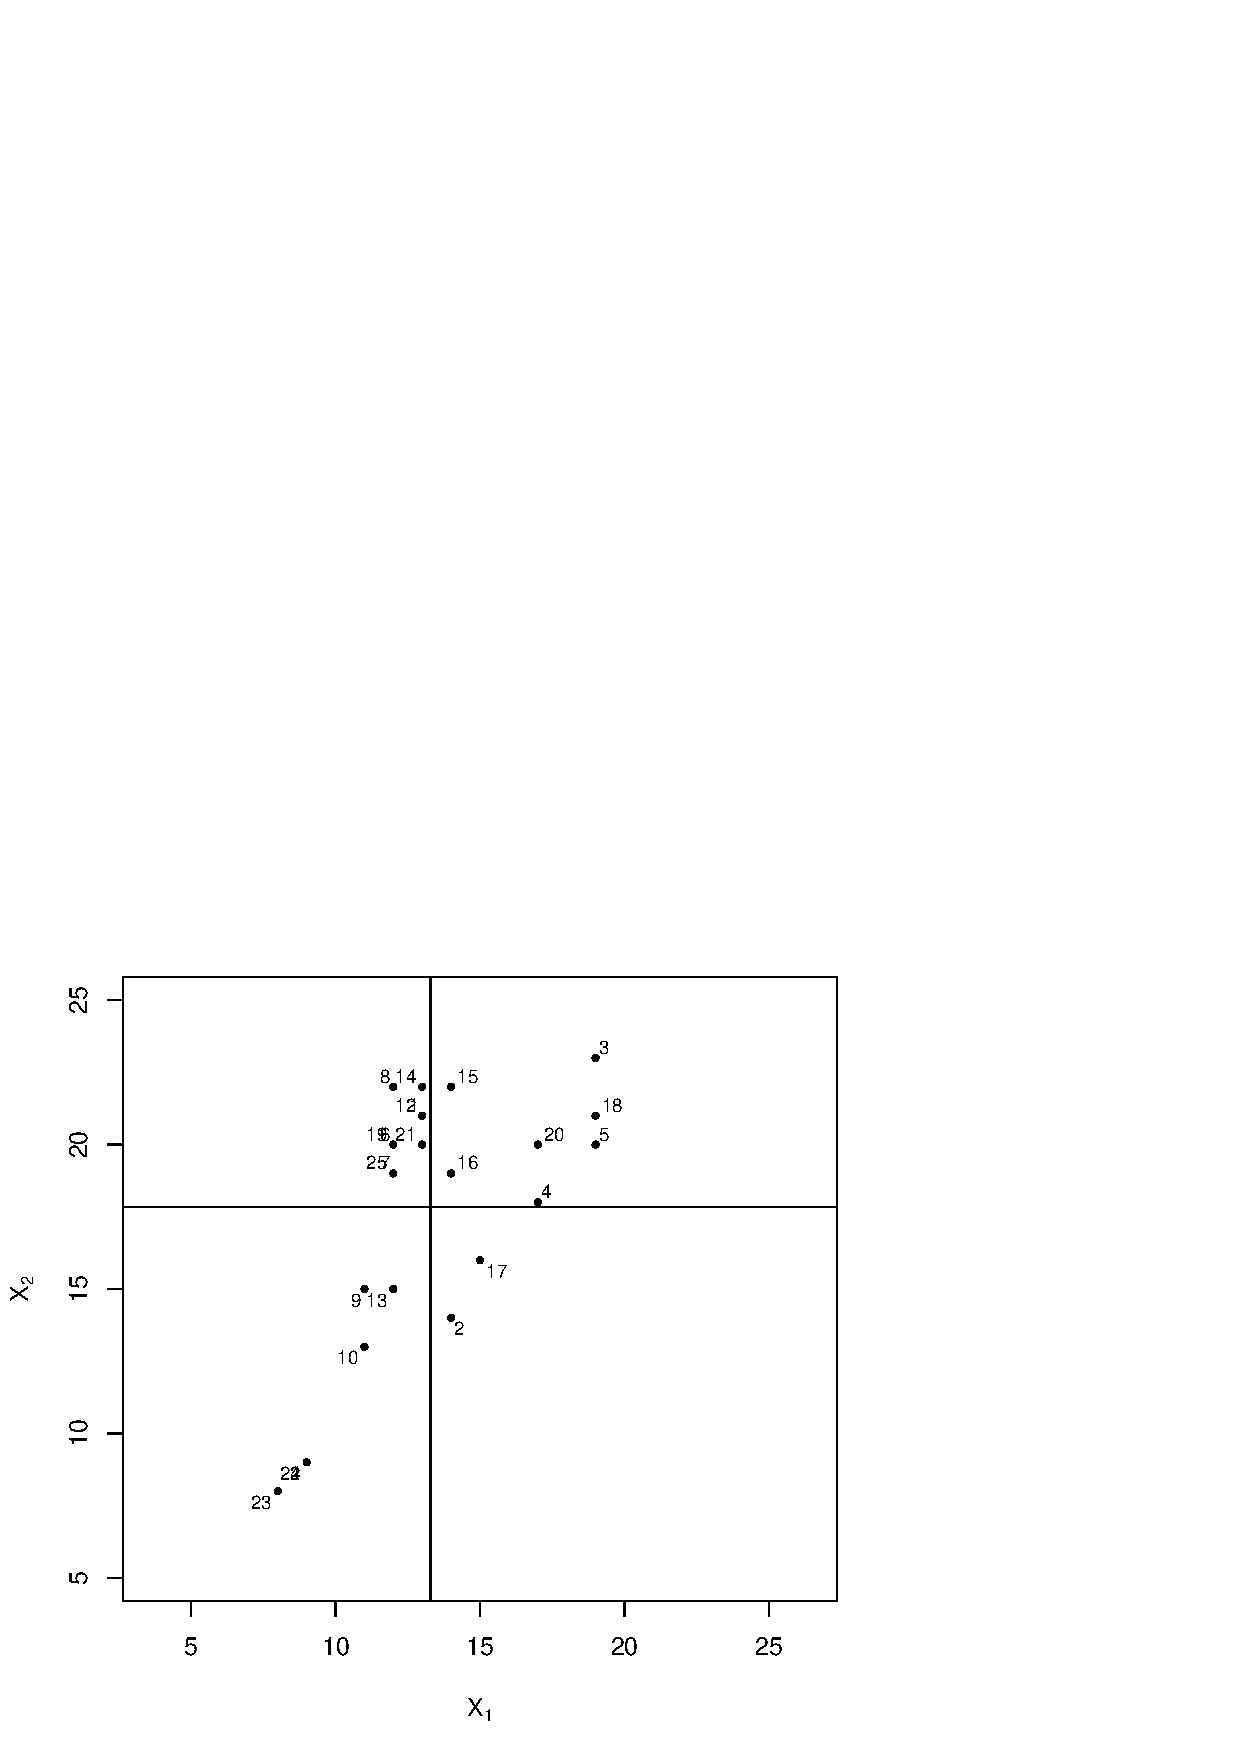
\includegraphics{CalibrationGuide-004}

Next, we perform the regression of $X_5$ onto $X_1$ and $X_2$ (all variables being centered) in order to 
obtain an additional axis for $X_5$. We represent $X_5$ in the plot as a simple 
arrow whose coordinates are given by the regression coefficients:

\begin{Schunk}
\begin{Sinput}
> Xc <- scale(X, center = T, scale = F)
> b <- solve(t(Xc[, 1:2]) %*% Xc[, 1:2]) %*% t(Xc[, 
+     1:2]) %*% Xc[, 5]
> print(b)
\end{Sinput}
\begin{Soutput}
        [,1]
X1 0.3850425
X2 0.1225419
\end{Soutput}
\begin{Sinput}
> bscaled <- 20 * b
> arrows(m[1], m[2], m[1] + bscaled[1], m[2] + bscaled[2], 
+     col = "blue", length = 0.1)
> arrows(m[1], m[2], m[1] - bscaled[1], m[2] - bscaled[2], 
+     length = 0, lty = "dashed", col = "blue")
\end{Sinput}
\end{Schunk}
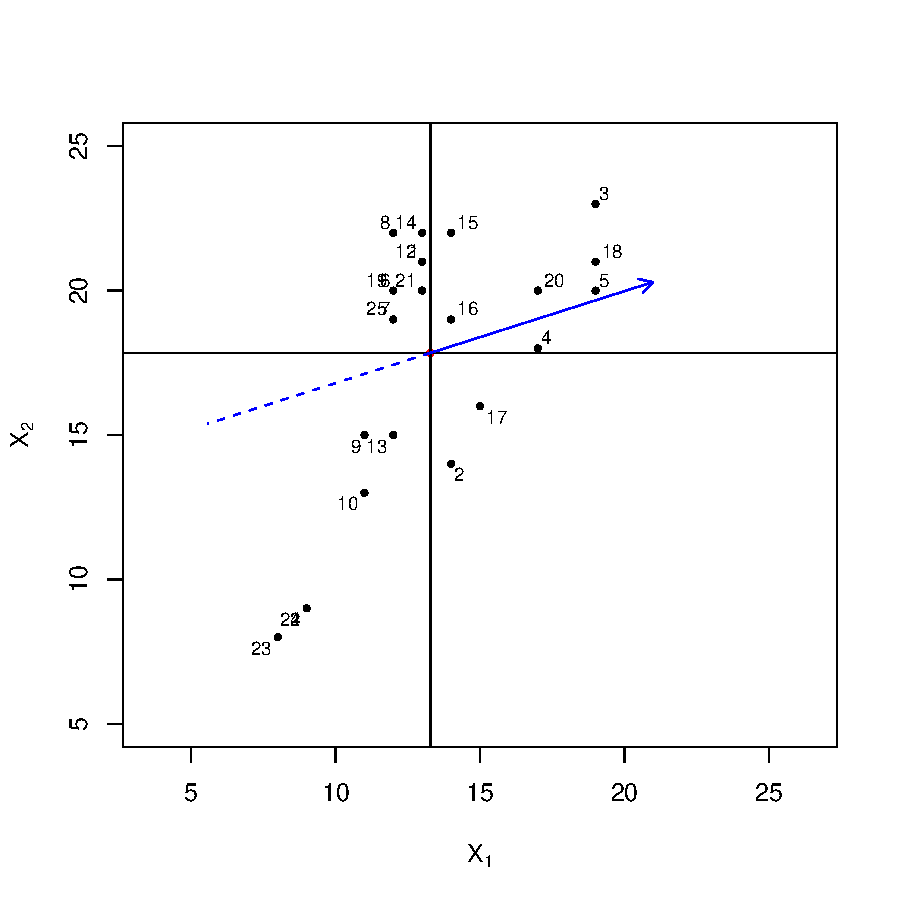
\includegraphics{CalibrationGuide-005}

A direction that is optimal in the least squares sense for $X_5$ is given by the vector of regression
coefficients~(2003). To make this direction more visible, we multiplied it by a constant (20). 
It is clear that the direction of increase for $X_5$ runs approximately North-East across the scatterplot. 
We now proceed to calibrate this direction with a scale for $X_5$. In order to choose sensible values for
the scale of $X_5$, we first inspect the range of variation of $X_5$, and then choose a set of values we want
to mark off on the scale ({\tt tm}) and also compute the deviations of these values from the mean 
({\tt tmc}). We specify a tick length of 0.3 ({\tt tl=0.3}). Depending on the data, some values of {\tt tl}
typically have to be tried to see how to obtain a nice scale. 

\begin{Schunk}
\begin{Sinput}
> print(range(X[, 5]))
\end{Sinput}
\begin{Soutput}
[1]  2 11
\end{Soutput}
\begin{Sinput}
> yc <- scale(X[, 5], scale = F)
> tm <- seq(2, 10, by = 1)
> tmc <- tm - mean(X[, 5])
> Calibrate.X5 <- calibrate(b, yc, tmc, Xc[, 1:2], 
+     tmlab = tm, m = m, tl = 0.3, axislab = "X_5", 
+     labpos = 4, cex.axislab = 1)
\end{Sinput}
\begin{Soutput}
---------- Calibration Results for  X_5  -------------------
Length of 1 unit of the original variable =  2.4748  
Angle                                     =  17.65 degrees
Optimal calibration factor                =  6.1247  
Used calibration factor                   =  6.1247  
Goodness-of-fit                           =  0.5133  
Goodness-of-scale                         =  0.5133  
------------------------------------------------------------
\end{Soutput}
\end{Schunk}
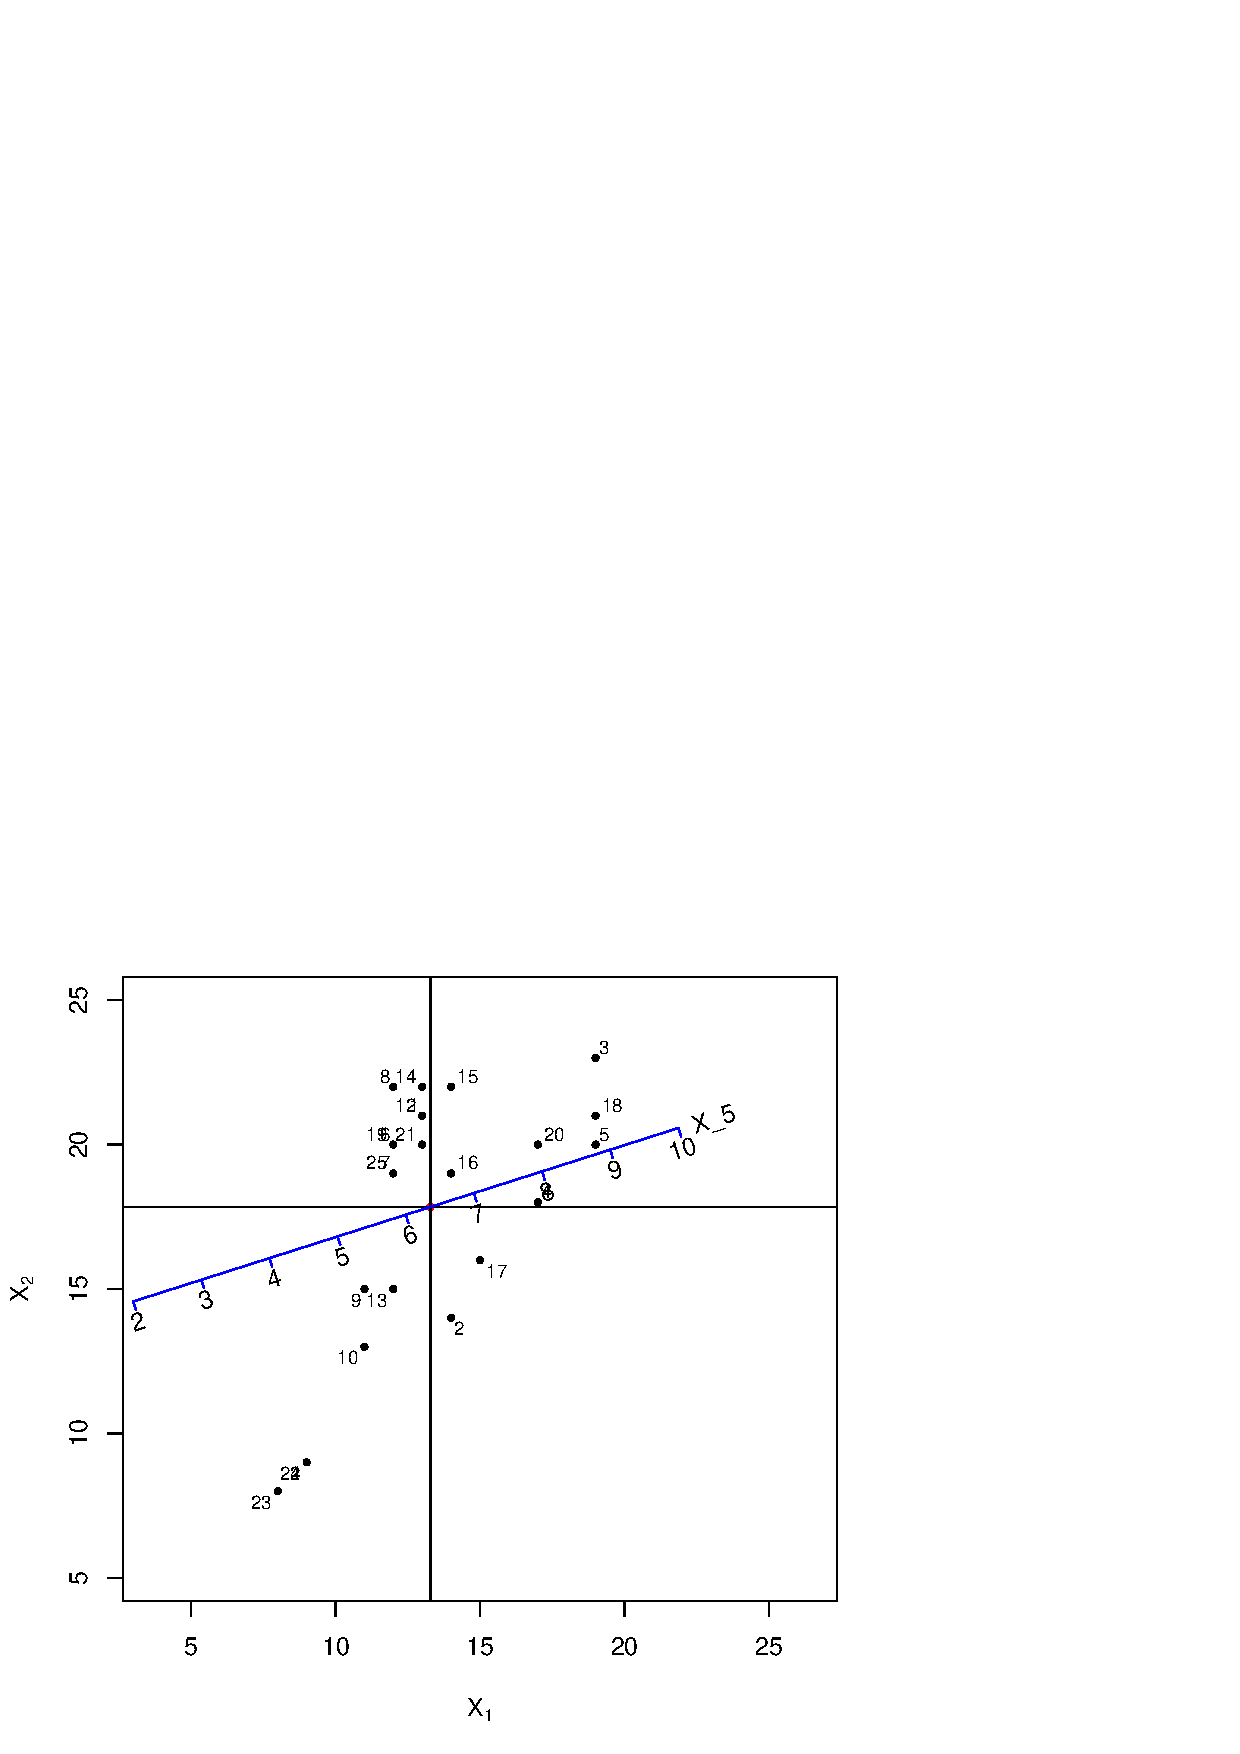
\includegraphics{CalibrationGuide-006}

The numerical output from routine {\tt calibrate} shows that one unit along the axis for $X_5$ occupies 2.47
units in the plotting frame. The axis for $X_5$ makes an angle of 17.65 degrees with the positive x-axis.
The calibration factor is 6.12. Multiplying the vector of regressions coefficients by this
factor yields a vector that represents a unit change in the scale of $X_5$. E.g. for this data we have that 
the vector $6.12 \cdot (0.385, 0.123) = (2.358, 0.751)$ represents a unit change. This vector has
norm $\sqrt{2.358^2 + 0.751^2} = 2.47$. Other calibration factors may be specified by using parameter
{\tt alpha}. If {\tt alpha} is left unspecified the optimal value computed by least
squares will be used. The goodness-of-fit of $X_5$ is 0.513. This means that 51.3\% of the variance
of $X_5$ can be explained by a regression onto $X_1$ and $X_2$ ($R^2 = 0.513$). The goodness-of-scale has
the same value. The goodness-of-scale is only relevant if we modify parameter {\tt alpha}. {\tt Calibrate.X5}
is a list object containing all calibration results (calibration factor, fitted values according to the
scale used, tick marker positions, etc.)

\subsubsection*{Second vertical axis in a scatterplot}

The oblique direction in the previous section is the preferred direction for $X_5$, as this direction
is optimal in the least squares sense. However, if desired, additional variables can also be represented
as a second vertical axis on the right of the plot, or as a second horizontal axis on the top of the
plot. We now proceed to construct a second vertical axis on the right hand of the scatter plot for
$X_5$. This can be done by setting the vector to be calibrated (first argument of routine {\tt calibrate})
to the (0,1) vector. By specifying a {\tt shift} factor, the axis can be shifted. For this data, setting
the {\tt shift} value to {\tt par('usr')[2]-mean(X[,1])} will make the axis coincide with the right vertical
borderline of the graph.

\begin{Schunk}
\begin{Sinput}
> opar <- par(xpd = T)
> tm <- seq(3, 8, by = 1)
> tmc <- (tm - mean(X[, 5]))
> Calibrate.rightmargin.X5 <- calibrate(c(0, 1), 
+     yc, tmc, Xc[, 1:2], tmlab = tm, m = m, axislab = "X_5", 
+     tl = 0.5, shift = par("usr")[2] - mean(X[, 
+         1]), where = 2, laboffset = c(1.5, 1.5), 
+     cex.axislab = 1)
\end{Sinput}
\begin{Soutput}
---------- Calibration Results for  X_5  -------------------
Length of 1 unit of the original variable =  3.4603  
Angle                                     =  90 degrees
Optimal calibration factor                =  3.4603  
Used calibration factor                   =  3.4603  
Goodness-of-fit                           =  0.3373  
Goodness-of-scale                         =  0.3373  
------------------------------------------------------------
\end{Soutput}
\begin{Sinput}
> par(opar)
\end{Sinput}
\end{Schunk}
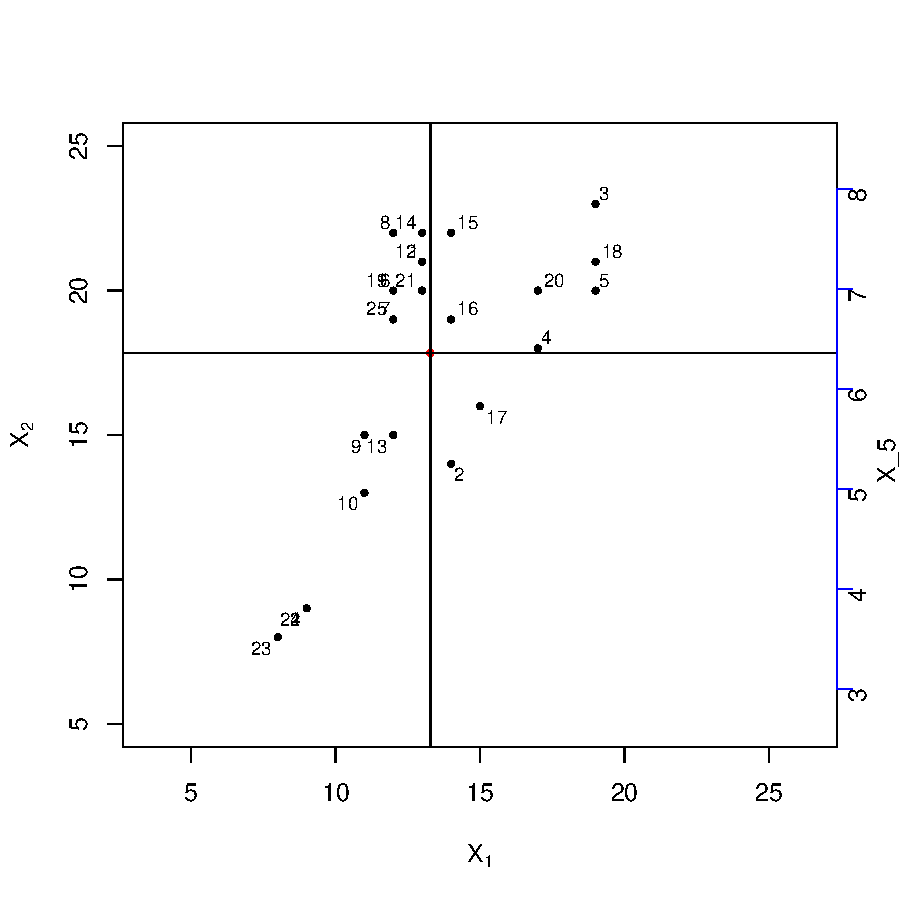
\includegraphics{CalibrationGuide-007}

The second vertical axis has calibration factor 3.46, and a goodness of fit of 0.34. The fit of the
variable is worse in comparison with the previous oblique direction given by the regression coefficients. Note
that graphical clipping in temporarily turned off ({\tt par('xpd'=T)}) to allow the calibration 
routine to draw ticks and labels outside the figure region, and that the range of the tick marks was
shortened in order not surpass the figure region.
\clearpage

\subsubsection*{Subscales and double calibrations}

Scales with tick marks can be refined by drawing subscales with smaller tick marks. 
E.g. larger labelled
tickmarks can be used to represent multiples of 10, and small unlabelled tick marks can be used to 
represent units. The subscale allows a more precise recovery of the data values. This can simply be 
achieved by calling the calibration routine twice, once with a coarse sequence and once with a finer 
sequence. For the second call one can specify {\tt verb=F} in order to suppress the numerical output
of the routine, and {\tt lm=F} to supress the tick mark labels under the smaller ticks. The tickmarks
for the finer scale are made smaller by modifying the tick length (e.g. {\tt tl=0.1}). Depending on the data, 
some trial and error with different values for {\tt tl} may be necessary before nice scales are obtained. This
may be automatized in the future. Finally, reading off the (approximate) data values can further be enhanced 
by drawing perpendiculars from the points to the calibrated axis by setting {\tt dp=T}.

\begin{Schunk}
\begin{Sinput}
> tm <- seq(2, 10, by = 1)
> tmc <- (tm - mean(X[, 5]))
> Calibrate.X5 <- calibrate(b, yc, tmc, Xc[, 1:2], 
+     tmlab = tm, m = m, axislab = "X_5", tl = 0.5, 
+     dp = T, labpos = 4)
\end{Sinput}
\begin{Soutput}
---------- Calibration Results for  X_5  -------------------
Length of 1 unit of the original variable =  2.4748  
Angle                                     =  17.65 degrees
Optimal calibration factor                =  6.1247  
Used calibration factor                   =  6.1247  
Goodness-of-fit                           =  0.5133  
Goodness-of-scale                         =  0.5133  
------------------------------------------------------------
\end{Soutput}
\begin{Sinput}
> tm <- seq(2, 10, by = 0.1)
> tmc <- (tm - mean(X[, 5]))
> Calibrate.X5 <- calibrate(b, yc, tmc, Xc[, 1:2], 
+     tmlab = tm, m = m, tl = 0.25, verb = F, lm = F)
\end{Sinput}
\end{Schunk}
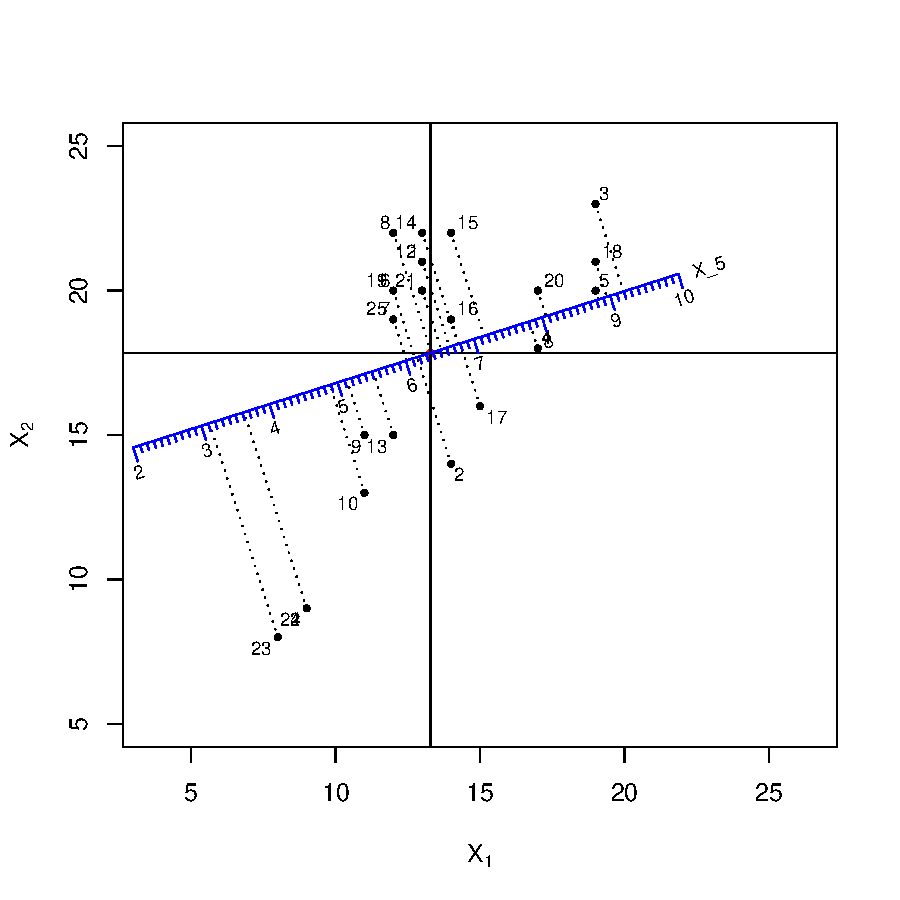
\includegraphics{CalibrationGuide-008}

A {\it double calibration} can be created by drawing two scales, one on each side of the axis. Double
calibrations can be useful. For instance, one scale can be used for recovery of the original 
data values of the variable, whereas the second scale can be used for recovery of standardized values or
of correlations with other variables. Double calibrations can also be used to 
graphically verify if two different calibration procedures give the same result or not. 

\subsubsection*{Recalibrating the original scatterplot axes}

By calibrating the (0,1) and (1,0) vectors the original axes of the scatter plot can be 
redesigned. We illustrate the recalibration of the original axes by creating a second scale on
the other side of the axes, a refined scale for $X_1$, and a scale for the standardized data for
$X_2$. For the latter calibration one unit equals one standard deviation. 

\begin{Schunk}
\begin{Sinput}
> opar <- par(xpd = T)
> tm <- seq(5, 25, by = 5)
> tmc <- (tm - mean(X[, 1]))
> yc <- scale(X[, 1], scale = F)
> Calibrate.X1 <- calibrate(c(1, 0), yc, tmc, Xc[, 
+     1:2], tmlab = tm, m = m, tl = 0.5, axislab = "X_1", 
+     cex.axislab = 1, showlabel = F, shift = -(mean(X[, 
+         2]) - par("usr")[3])^2, reverse = T)
\end{Sinput}
\begin{Soutput}
---------- Calibration Results for  X_1  -------------------
Length of 1 unit of the original variable =  1  
Angle                                     =  0 degrees
Optimal calibration factor                =  1  
Used calibration factor                   =  1  
Goodness-of-fit                           =  1  
Goodness-of-scale                         =  1  
------------------------------------------------------------
\end{Soutput}
\begin{Sinput}
> tm <- seq(5, 25, by = 1)
> tmc <- (tm - mean(X[, 1]))
> Calibrate.X1 <- calibrate(c(1, 0), yc, tmc, Xc[, 
+     1:2], tmlab = tm, m = m, tl = 0.25, axislab = "X_1", 
+     cex.axislab = 1, showlabel = F, shift = -(mean(X[, 
+         2]) - par("usr")[3])^2, reverse = T, verb = F, 
+     lm = F)
> yc <- scale(X[, 2], scale = T)
> tm <- seq(-3, 1, by = 1)
> Calibrate.X2 <- calibrate(c(0, 1), yc, tm, Xc[, 
+     1:2], tmlab = tm, m = m, tl = 0.6, axislab = "X_2", 
+     cex.axislab = 1, showlabel = F, shift = -(mean(X[, 
+         1]) - par("usr")[1]), verb = T, lm = T)
\end{Sinput}
\begin{Soutput}
---------- Calibration Results for  X_2  -------------------
Length of 1 unit of the original variable =  4.3367  
Angle                                     =  90 degrees
Optimal calibration factor                =  4.3367  
Used calibration factor                   =  4.3367  
Goodness-of-fit                           =  1  
Goodness-of-scale                         =  1  
------------------------------------------------------------
\end{Soutput}
\begin{Sinput}
> tm <- seq(-3, 1.5, by = 0.1)
> Calibrate.X2 <- calibrate(c(0, 1), yc, tm, Xc[, 
+     1:2], tmlab = tm, m = m, tl = 0.3, axislab = "X_2", 
+     cex.axislab = 1, showlabel = F, shift = -(mean(X[, 
+         1]) - par("usr")[1]), verb = F, lm = F)
> par(opar)
\end{Sinput}
\end{Schunk}
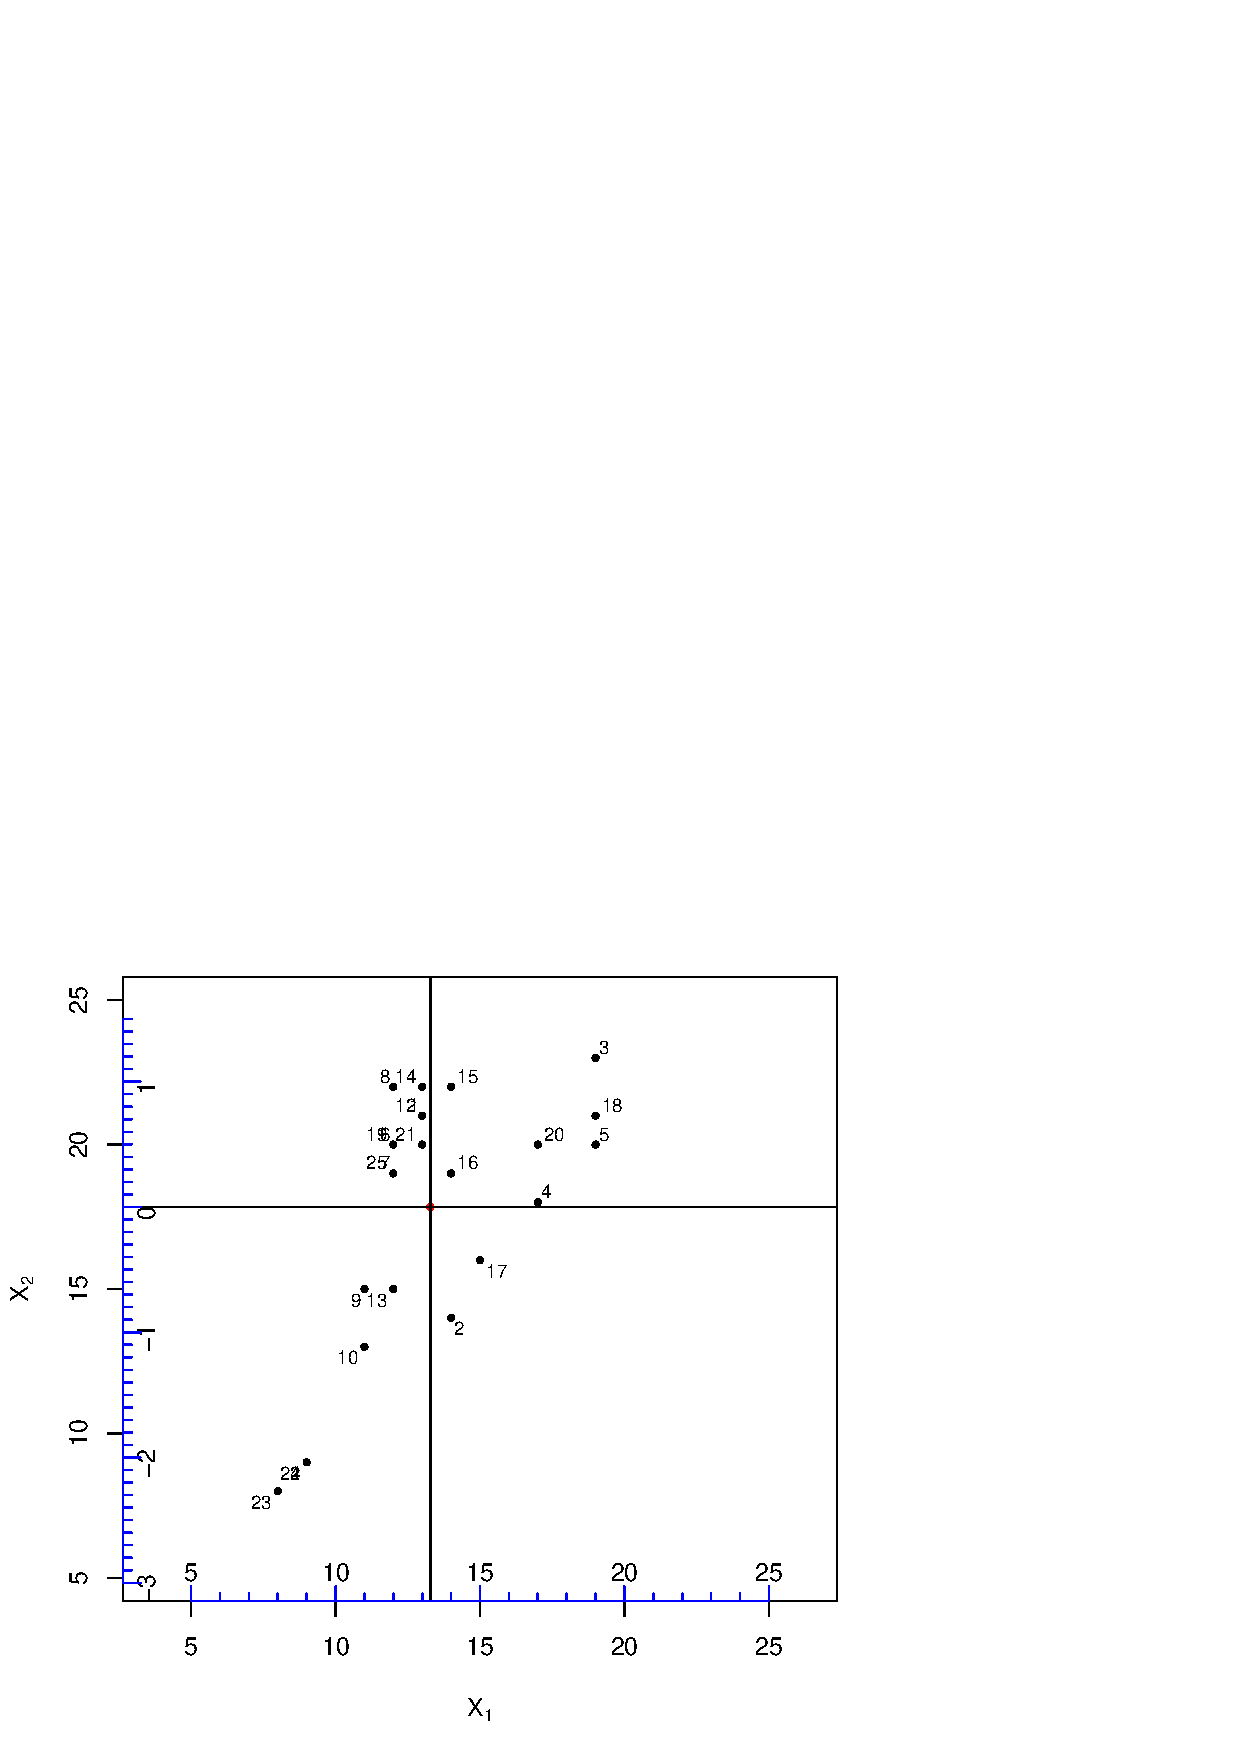
\includegraphics{CalibrationGuide-009}

\section{Calibration of Biplot axes}
\label{sec:biplot}

In this section we give detailed instructions on how to calibrate biplot axes. We will consider biplots 
of raw data matrices and correlation matrices obtained by PCA, biplots of profiles obtained in CA,
biplots of data matrices and correlation matrices (in particular the between-set correlation matrix) 
in CCA and biplots of fitted values and regression coefficients obtained by RDA. In principle, calibration
of biplot axes has little additional complication in comparison with the calibration of additional 
axes in scatterplots explained above. The main issue is that, prior to calling the calibration routine,
one needs to take care of the proper centring and standardisation of the tick marks. 

\subsection{Principal component analysis}
\label{sec:pca}

Principal component analysis can be performed by using routine {\tt princomp} from the {\tt stats }
library. We use again Manly's goblets data to create a biplot of the data based on a
PCA of the covariance matrix. We use {\tt princomp} to compute the scores for the rows and the columns
of the data matrix. The first principal component is seen to be a size component, separating the
smaller goblets on the right from the larger goblets on the left. The variable vectors are 
multiplied by a factor of 15 to facilitate interpretation. Next  we 
calibrate the vector for $X_3$, 
using labelled tickmarks for multiples of 5 units, and shorter unlabelled tickmarks for the units. The 
goodness of fit of $X_3$ is very high (0.99), which means that $X_3$ is close to perfectly 
represented. {\tt Calibrate.X3} is a list object containing the numerical results of the 
calibration.

\begin{Schunk}
\begin{Sinput}
> pca.results <- princomp(X, cor = F)
> Fp <- pca.results$scores
> Gs <- pca.results$loadings
> plot(Fp[, 1], Fp[, 2], pch = 16, asp = 1, xlab = "PC 1", 
+     ylab = "PC 2", cex = 0.5)
> textxy(Fp[, 1], Fp[, 2], rownames(X), cx = 0.75)
> arrows(0, 0, 15 * Gs[, 1], 15 * Gs[, 2], length = 0.1)
> textxy(15 * Gs[, 1], 15 * Gs[, 2], colnames(X), 
+     cx = 0.75)
> ticklab <- seq(5, 30, by = 5)
> ticklabc <- ticklab - mean(X[, 3])
> yc <- (X[, 3] - mean(X[, 3]))
> g <- Gs[3, 1:2]
> Calibrate.X3 <- calibrate(g, yc, ticklabc, Fp[, 
+     1:2], ticklab, tl = 0.5, axislab = "X3", cex.axislab = 0.75, 
+     where = 1, labpos = 4)
\end{Sinput}
\begin{Soutput}
---------- Calibration Results for  X3  --------------------
Length of 1 unit of the original variable =  1.1813  
Angle                                     =  39.28 degrees
Optimal calibration factor                =  1.3954  
Used calibration factor                   =  1.3954  
Goodness-of-fit                           =  0.9914  
Goodness-of-scale                         =  0.9914  
------------------------------------------------------------
\end{Soutput}
\begin{Sinput}
> ticklab <- seq(5, 30, by = 1)
> ticklabc <- ticklab - mean(X[, 3])
> Calibrate.X3.fine <- calibrate(g, yc, ticklabc, 
+     Fp[, 1:2], ticklab, lm = F, tl = 0.25, verb = F, 
+     cex.axislab = 0.75, where = 1, labpos = 4)
\end{Sinput}
\end{Schunk}
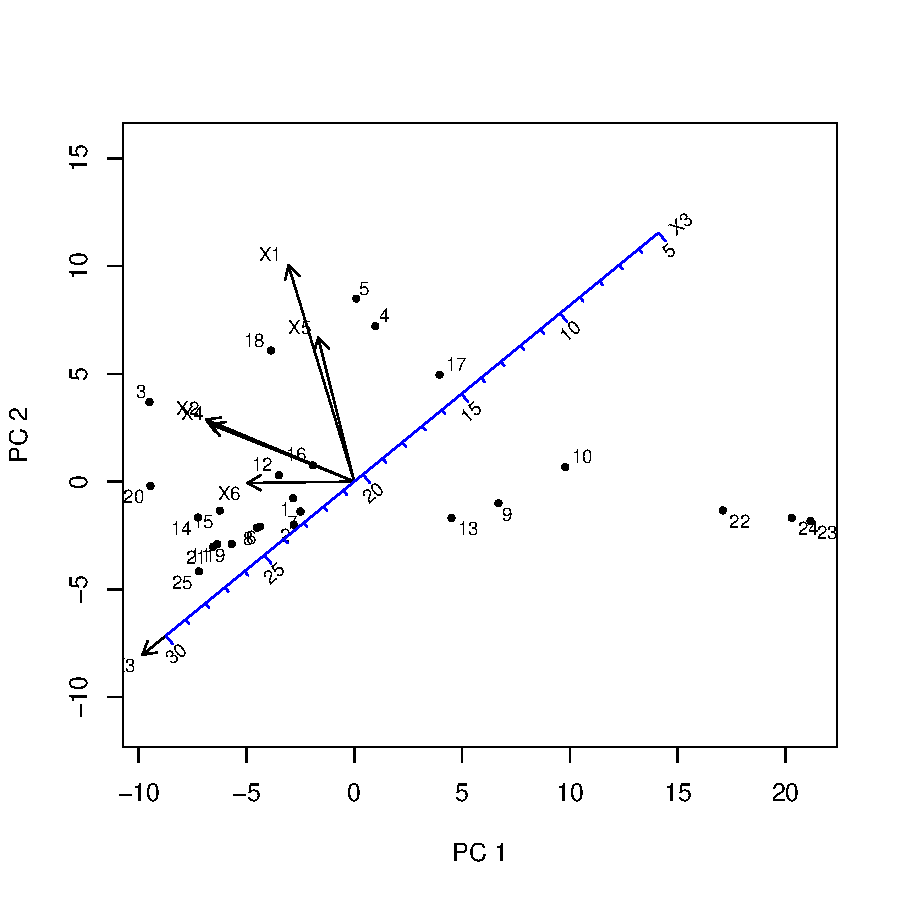
\includegraphics{CalibrationGuide-010}

We do a PCA based on the correlation matrix, and proceed to construct a biplot of the correlation matrix. The
correlations of $X_5$ with the other variables are computed, and the biplot axis for $X_5$ is calibrated with a 
correlation scale. Routine {\tt calibrate} is repeatedly called to create finer subscales.

\begin{Schunk}
\begin{Sinput}
> pca.results <- princomp(X, cor = T)
> Fp <- pca.results$scores
> Ds <- diag(pca.results$sdev)
> Fs <- Fp %*% solve(Ds)
> Gs <- pca.results$loadings
> Gp <- Gs %*% Ds
> plot(Gp[, 1], Gp[, 2], pch = 16, cex = 0.5, xlim = c(-1, 
+     1), ylim = c(-1, 1), asp = 1, xlab = "1st principal axis", 
+     ylab = "2nd principal axis")
> arrows(0, 0, Gp[, 1], Gp[, 2], length = 0.1)
> textxy(Gp[, 1], Gp[, 2], colnames(X), cx = 0.75)
> ticklab <- c(seq(-1, -0.2, by = 0.2), seq(0.2, 
+     1, by = 0.2))
> R <- cor(X)
> y <- R[, 5]
> g <- Gp[5, 1:2]
> Calibrate.X5 <- calibrate(g, y, ticklab, Gp[, 
+     1:2], ticklab, lm = T, tl = 0.05, dp = T, 
+     labpos = 2, cex.axislab = 0.75, axislab = "X_5")
\end{Sinput}
\begin{Soutput}
---------- Calibration Results for  X_5  -------------------
Length of 1 unit of the original variable =  1.0634  
Angle                                     =  -49.36 degrees
Optimal calibration factor                =  1.1308  
Used calibration factor                   =  1.1308  
Goodness-of-fit                           =  0.9824  
Goodness-of-scale                         =  0.9824  
------------------------------------------------------------
\end{Soutput}
\begin{Sinput}
> ticklab <- seq(-1, 1, by = 0.1)
> Calibrate.X5 <- calibrate(g, y, ticklab, Gp[, 
+     1:2], ticklab, lm = F, tl = 0.05, verb = F)
> ticklab <- seq(-1, 1, by = 0.01)
> Calibrate.X5 <- calibrate(g, y, ticklab, Gp[, 
+     1:2], ticklab, lm = F, tl = 0.025, verb = F)
\end{Sinput}
\end{Schunk}
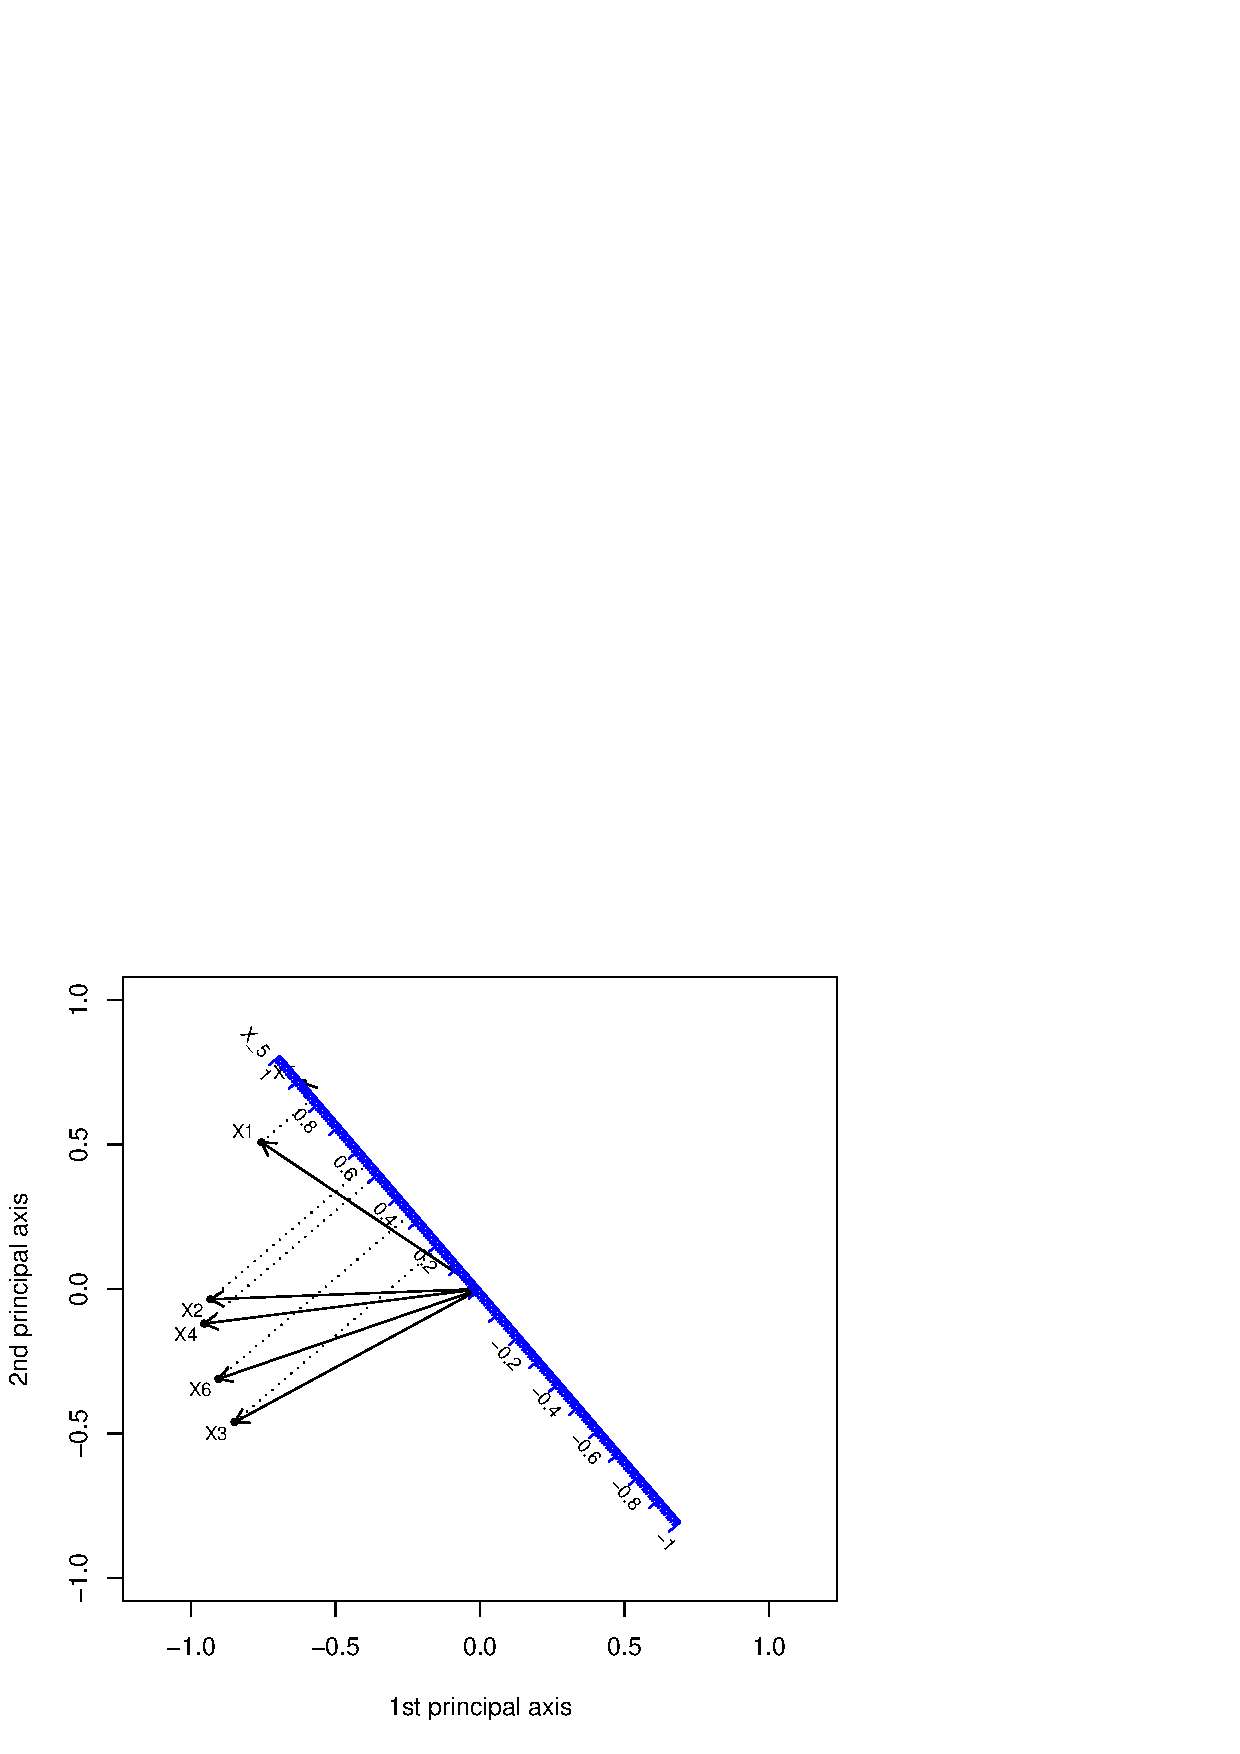
\includegraphics{CalibrationGuide-011}

The goodness of fit of the representation of the correlations of $X_5$ with the
other variables is 0.98, the 6 correlations being close to perfectly represented.
We compute the sample correlation matrix and compare the observed correlations of 
$X_5$ with those estimated from the calibrated biplot axis ({\tt yt}). Note that
PCA also tries to approximate the correlation of a variable with itself, and that
the arrow on representing $X_5$ falls short of the value 1 on its own calibrated scale.
The refined subscale allows very precise graphical representation of the correlations
as estimated by the biplot.

\begin{center}
\begin{Schunk}
\begin{Sinput}
> print(R)
\end{Sinput}
\begin{Soutput}
          X1        X2        X3        X4        X5
X1 1.0000000 0.6234051 0.3464089 0.6748429 0.6901040
X2 0.6234051 1.0000000 0.8392292 0.8287898 0.5807725
X3 0.3464089 0.8392292 1.0000000 0.8430518 0.2511584
X4 0.6748429 0.8287898 0.8430518 1.0000000 0.4874610
X5 0.6901040 0.5807725 0.2511584 0.4874610 1.0000000
X6 0.5875703 0.7970192 0.8575089 0.9101886 0.2885165
          X6
X1 0.5875703
X2 0.7970192
X3 0.8575089
X4 0.9101886
X5 0.2885165
X6 1.0000000
\end{Soutput}
\begin{Sinput}
> print(cbind(R[, 5], Calibrate.X5$yt))
\end{Sinput}
\begin{Soutput}
        [,1]      [,2]
X1 0.6901040 0.8257486
X2 0.5807725 0.5462001
X3 0.2511584 0.1914136
X4 0.4874610 0.4992765
X5 1.0000000 0.8843474
X6 0.2885165 0.3326711
\end{Soutput}
\end{Schunk}
\end{center}

\subsection{Correspondence analysis}
\label{sec:ca}

We consider a contingency table of a sample of Dutch calves born in the late nineties,
shown in Table~\ref{tab:calves2}. A total of 7257 calves were classified according 
to two categorical variables: the
method of production (ET = Embryo Transfer, IVP = In Vitro Production, AI = Artificial
Insemination) and the ease of delivery, scored on a scale from 1 (normal) to 6 (very heavy).
The data in Table~\ref{tab:calves2} were provided by Holland Genetics.
\begin{table}[htb]
\centering
\begin{tabular}{c|rrrr}
 & \multicolumn{3}{c}{Type of calf}\\
Ease of delivery  & ET & IVP & AI\\
\hline
1 &  97 & 150 & 1686\\
2 & 152 & 183 & 1339\\
3 & 377 & 249 & 1209\\
4 & 335 & 227 &  656\\
5 &  42 & 136 &  277\\
6 &   9 &  71 &   62\\
\hline
\end{tabular}
\caption{Calves data from Holland Genetics.}
\label{tab:calves2}
\end{table}

For this contingency table we obtain $\chi^2_{10} = 833.16$ with $p < 0.001$ and the null
hypothesis of no association between ease of delivery and type of calf has to be rejected. However, what is
the precise nature of this association? Correspondence analysis can be used to gain insight in the 
nature of this association. We use routine {\tt corresp} form the {\tt MASS} library~\cite{Venables}
to perform correspondence analysis and to obtain the coordinates for a biplot of the row profiles.
We compute the row profiles and then repeatedly call the calibration routine, each time with a
different set of {\tt ticklabs}.

\begin{Schunk}
\begin{Sinput}
> library(MASS)
> data(calves)
> ca.results <- corresp(calves, nf = 2)
> Fs <- ca.results$rscore
> Gs <- ca.results$cscore
> Ds <- diag(ca.results$cor)
> Fp <- Fs %*% Ds
> Gp <- Gs %*% Ds
> plot(Gs[, 1], Gs[, 2], pch = 16, asp = 1, cex = 0.5, 
+     xlab = "1st principal axis", ylab = "2nd principal axis")
> textxy(Gs[, 1], Gs[, 2], colnames(calves), cx = 0.75)
> points(Fp[, 1], Fp[, 2], pch = 16, cex = 0.5)
> textxy(Fp[, 1], Fp[, 2], rownames(calves), cx = 0.75)
> origin()
> arrows(0, 0, Gs[, 1], Gs[, 2])
> P <- as.matrix(calves/sum(calves))
> r <- apply(P, 1, sum)
> k <- apply(P, 2, sum)
> Dc <- diag(k)
> Dr <- diag(r)
> RP <- solve(Dr) %*% P
> print(RP)
\end{Sinput}
\begin{Soutput}
             ET        IVP        AI
[1,] 0.05018107 0.07759959 0.8722193
[2,] 0.09080048 0.10931900 0.7998805
[3,] 0.20544959 0.13569482 0.6588556
[4,] 0.27504105 0.18637110 0.5385878
[5,] 0.09230769 0.29890110 0.6087912
[6,] 0.06338028 0.50000000 0.4366197
\end{Soutput}
\begin{Sinput}
> CRP <- RP - ones(nrow(RP), 1) %*% t(k)
> TCRP <- CRP %*% solve(Dc)
> y <- TCRP[, 3]
> g <- Gs[3, 1:2]
> ticklab <- c(0, seq(0, 1, by = 0.2))
> ticklabs <- (ticklab - k[3])/k[3]
> Calibrate.AI <- calibrate(g, y, ticklabs, Fp[, 
+     1:2], ticklab, lm = T, tl = 0.1, weights = Dr, 
+     axislab = "AI", labpos = 4, dp = T)
\end{Sinput}
\begin{Soutput}
---------- Calibration Results for  AI  --------------------
Length of 1 unit of the original variable =  1.6057  
Angle                                     =  -6.82 degrees
Optimal calibration factor                =  2.5784  
Used calibration factor                   =  2.5784  
Goodness-of-fit                           =  1  
Goodness-of-scale                         =  1  
------------------------------------------------------------
\end{Soutput}
\begin{Sinput}
> ticklab <- c(0, seq(0, 1, by = 0.1))
> ticklabs <- (ticklab - k[3])/k[3]
> Calibrate.AI <- calibrate(g, y, ticklabs, Fp[, 
+     1:2], ticklab, lm = F, tl = 0.1, weights = Dr, 
+     verb = F)
> ticklab <- c(0, seq(0, 1, by = 0.01))
> ticklabs <- (ticklab - k[3])/k[3]
> Calibrate.AI <- calibrate(g, y, ticklabs, Fp[, 
+     1:2], ticklab, lm = F, tl = 0.05, weights = Dr, 
+     verb = F)
\end{Sinput}
\end{Schunk}
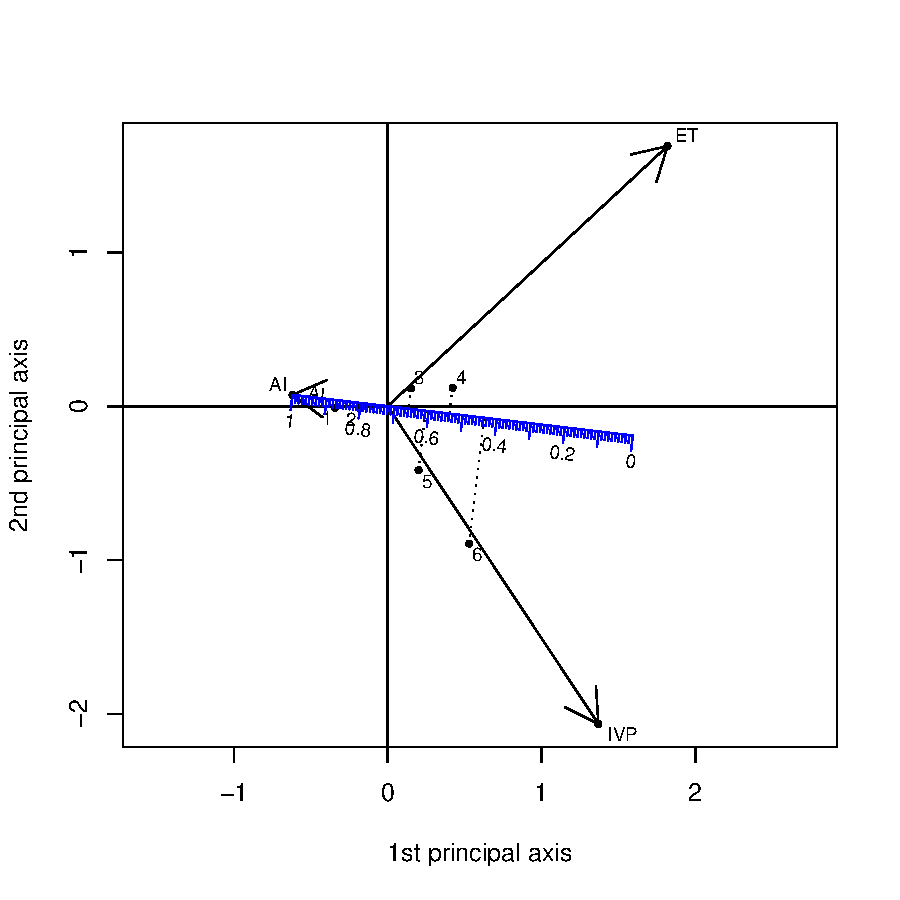
\includegraphics{CalibrationGuide-013}

Because the calibration is done by weighted least squares, a diagonal matrix of weights ({\tt weights=Dr}) 
is supplied as a parameter to the calibration routine
Note that the calibrated axis for the row profiles with respect to AI has goodness of fit 1. This
is due to the fact that the rank of the matrix of centred profiles is two, and that therefore
all profiles can be perfectly represented in two dimensional space.

\subsection{Canonical correlation analysis}
\label{sec:cca}

We consider a classical data set on the head sizes of the first and the second son of 25 families~\cite{Frets}.
These data have been analysed by several authors~\cite{Anderson,Mardia,Graffel16}
We first load the data and perform
a canonical correlation analysis, using supplied function {\tt canocor} (a more fully 
fledged program for canonical correlation analysis in comparison with {\tt cancor} from the {\tt stats} package).

\begin{Schunk}
\begin{Sinput}
> data(heads)
> X <- cbind(heads$X1, heads$X2)
> Y <- cbind(heads$Y1, heads$Y2)
> Rxy <- cor(X, Y)
> Ryx <- t(Rxy)
> Rxx <- cor(X)
> Ryy <- cor(Y)
> cca.results <- canocor(X, Y)
> plot(cca.results$Gs[, 1], cca.results$Gs[, 2], 
+     pch = 16, asp = 1, xlim = c(-1, 1), ylim = c(-1, 
+         1), xlab = expression(V[1]), ylab = expression(V[2]))
> arrows(0, 0, cca.results$Fp[, 1], cca.results$Fp[, 
+     2], length = 0.1)
> arrows(0, 0, cca.results$Gs[, 1], cca.results$Gs[, 
+     2], length = 0.1)
> textxy(cca.results$Fp[1, 1], cca.results$Fp[1, 
+     2], expression(X[1]), cx = 0.75)
> textxy(cca.results$Fp[2, 1], cca.results$Fp[2, 
+     2], expression(X[2]), cx = 0.75)
> textxy(cca.results$Gs[1, 1], cca.results$Gs[1, 
+     2], expression(Y[1]), cx = 0.75)
> textxy(cca.results$Gs[2, 1], cca.results$Gs[2, 
+     2], expression(Y[2]), cx = 0.75)
> circle(1)
\end{Sinput}
\begin{Soutput}
NULL
\end{Soutput}
\begin{Sinput}
> ticklab <- seq(-1, 1, by = 0.2)
> y <- Rxy[, 2]
> g <- cca.results$Gs[2, 1:2]
> Cal.Cor.Y2 <- calibrate(g, y, ticklab, cca.results$Fp[, 
+     1:2], ticklab, lm = T, tl = 0.05, dp = T, 
+     reverse = T, weights = solve(Rxx), axislab = "Y_2", 
+     cex.axislab = 0.75, showlabel = F)
\end{Sinput}
\begin{Soutput}
---------- Calibration Results for  Y_2  -------------------
Length of 1 unit of the original variable =  1  
Angle                                     =  -15.92 degrees
Optimal calibration factor                =  1  
Used calibration factor                   =  1  
Goodness-of-fit                           =  1  
Goodness-of-scale                         =  1  
------------------------------------------------------------
\end{Soutput}
\end{Schunk}
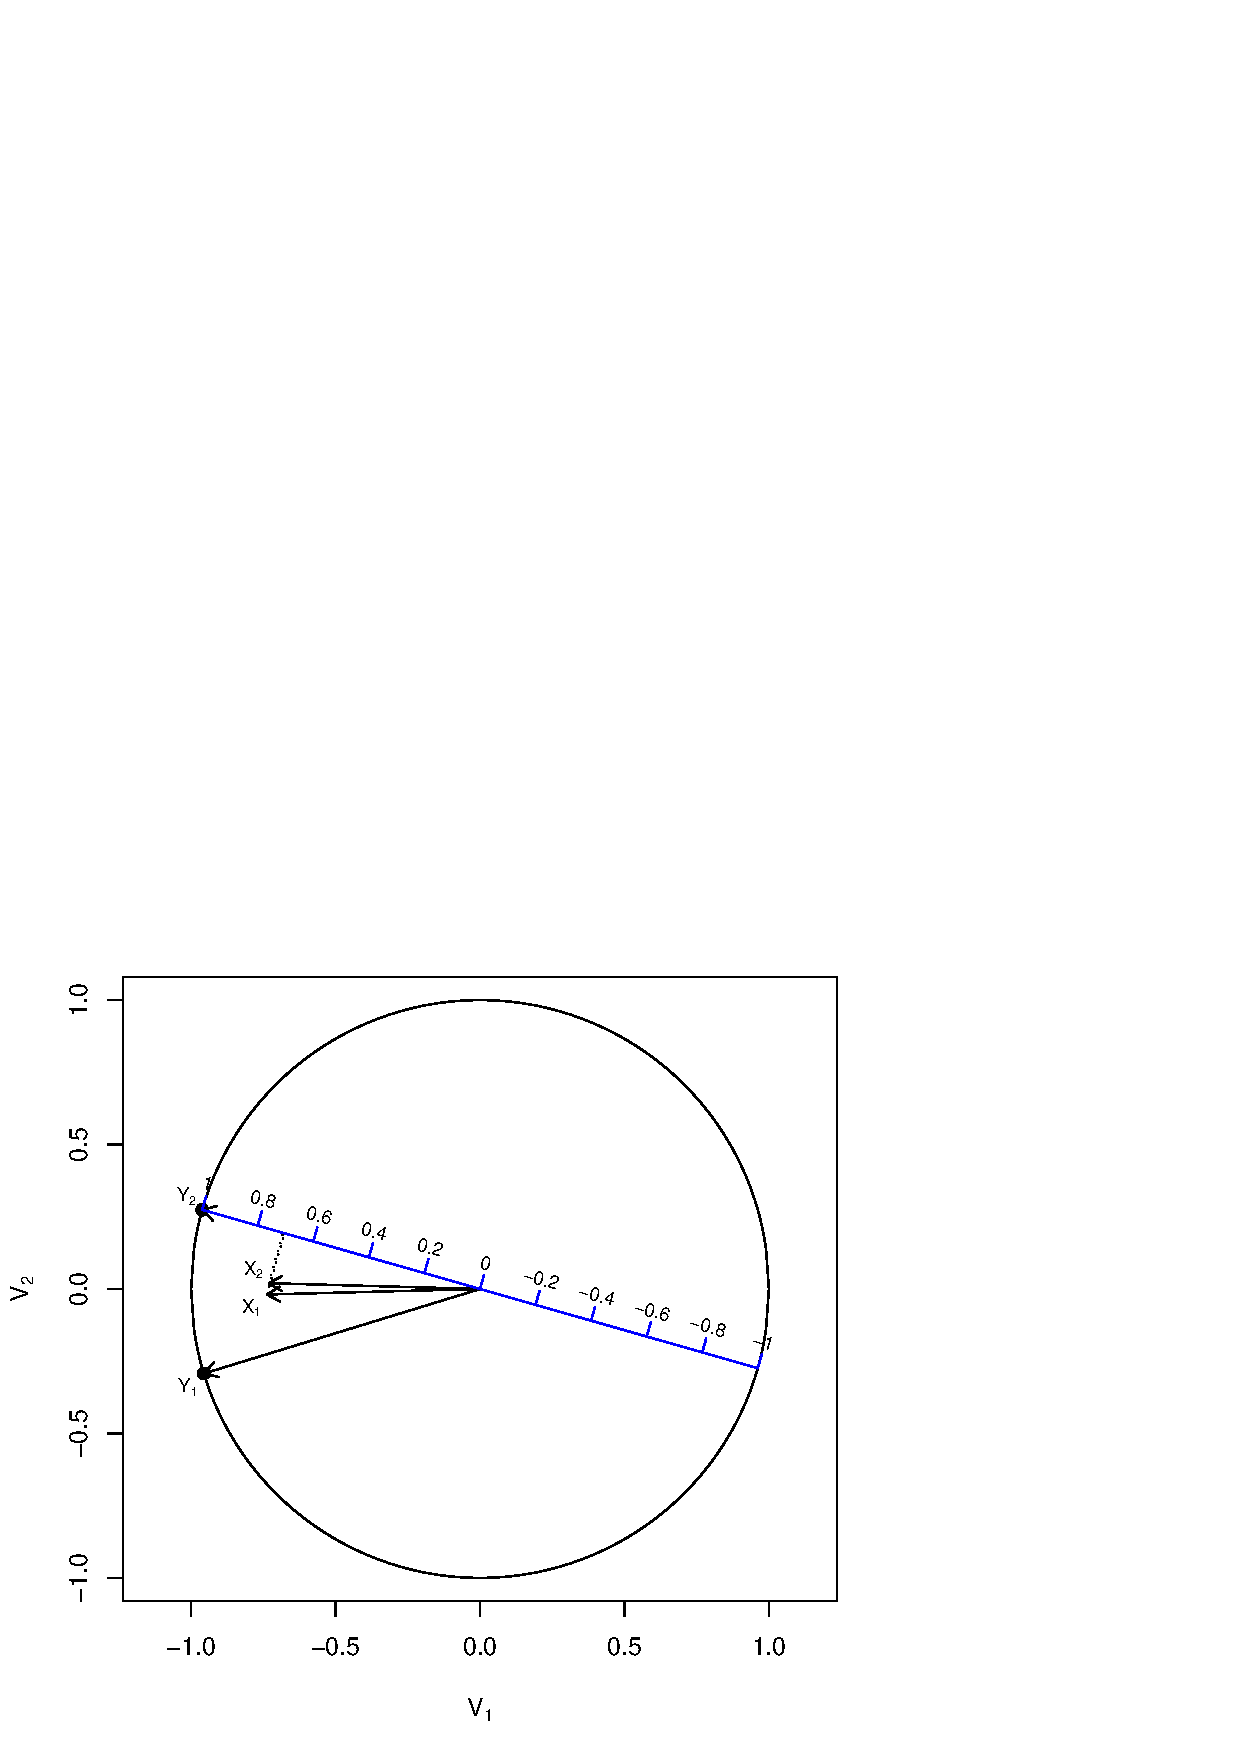
\includegraphics{CalibrationGuide-014}

\begin{Schunk}
\begin{Sinput}
> plot(cca.results$Gs[, 1], cca.results$Gs[, 2], 
+     pch = 16, asp = 1, xlim = c(-2, 2), ylim = c(-2, 
+         2), xlab = expression(V[1]), ylab = expression(V[2]))
> textxy(cca.results$Fp[1, 1], cca.results$Fp[1, 
+     2], expression(X[1]))
> textxy(cca.results$Fp[2, 1], cca.results$Fp[2, 
+     2], expression(X[2]))
> textxy(cca.results$Gs[1, 1], cca.results$Gs[1, 
+     2], expression(Y[1]))
> textxy(cca.results$Gs[2, 1], cca.results$Gs[2, 
+     2], expression(Y[2]))
> points(cca.results$V[, 1], cca.results$V[, 2], 
+     pch = 16, cex = 0.5)
> textxy(cca.results$V[, 1], cca.results$V[, 2], 
+     1:nrow(X), cx = 0.75)
> ticklab <- seq(135, 160, by = 5)
> ticklabc <- ticklab - mean(Y[, 2])
> ticklabs <- (ticklab - mean(Y[, 2]))/sqrt(var(Y[, 
+     2]))
> y <- (Y[, 2] - mean(Y[, 2]))/sqrt(var(Y[, 2]))
> Fr <- cca.results$V[, 1:2]
> g <- cca.results$Gs[2, 1:2]
> Cal.Data.Y2 <- calibrate(g, y, ticklabs, Fr, ticklab, 
+     lm = T, tl = 0.1, dp = T, reverse = T, verb = T, 
+     axislab = "Y_2", cex.axislab = 0.75, showlabel = F)
\end{Sinput}
\begin{Soutput}
---------- Calibration Results for  Y_2  -------------------
Length of 1 unit of the original variable =  1  
Angle                                     =  -15.92 degrees
Optimal calibration factor                =  1  
Used calibration factor                   =  1  
Goodness-of-fit                           =  1  
Goodness-of-scale                         =  1  
------------------------------------------------------------
\end{Soutput}
\end{Schunk}
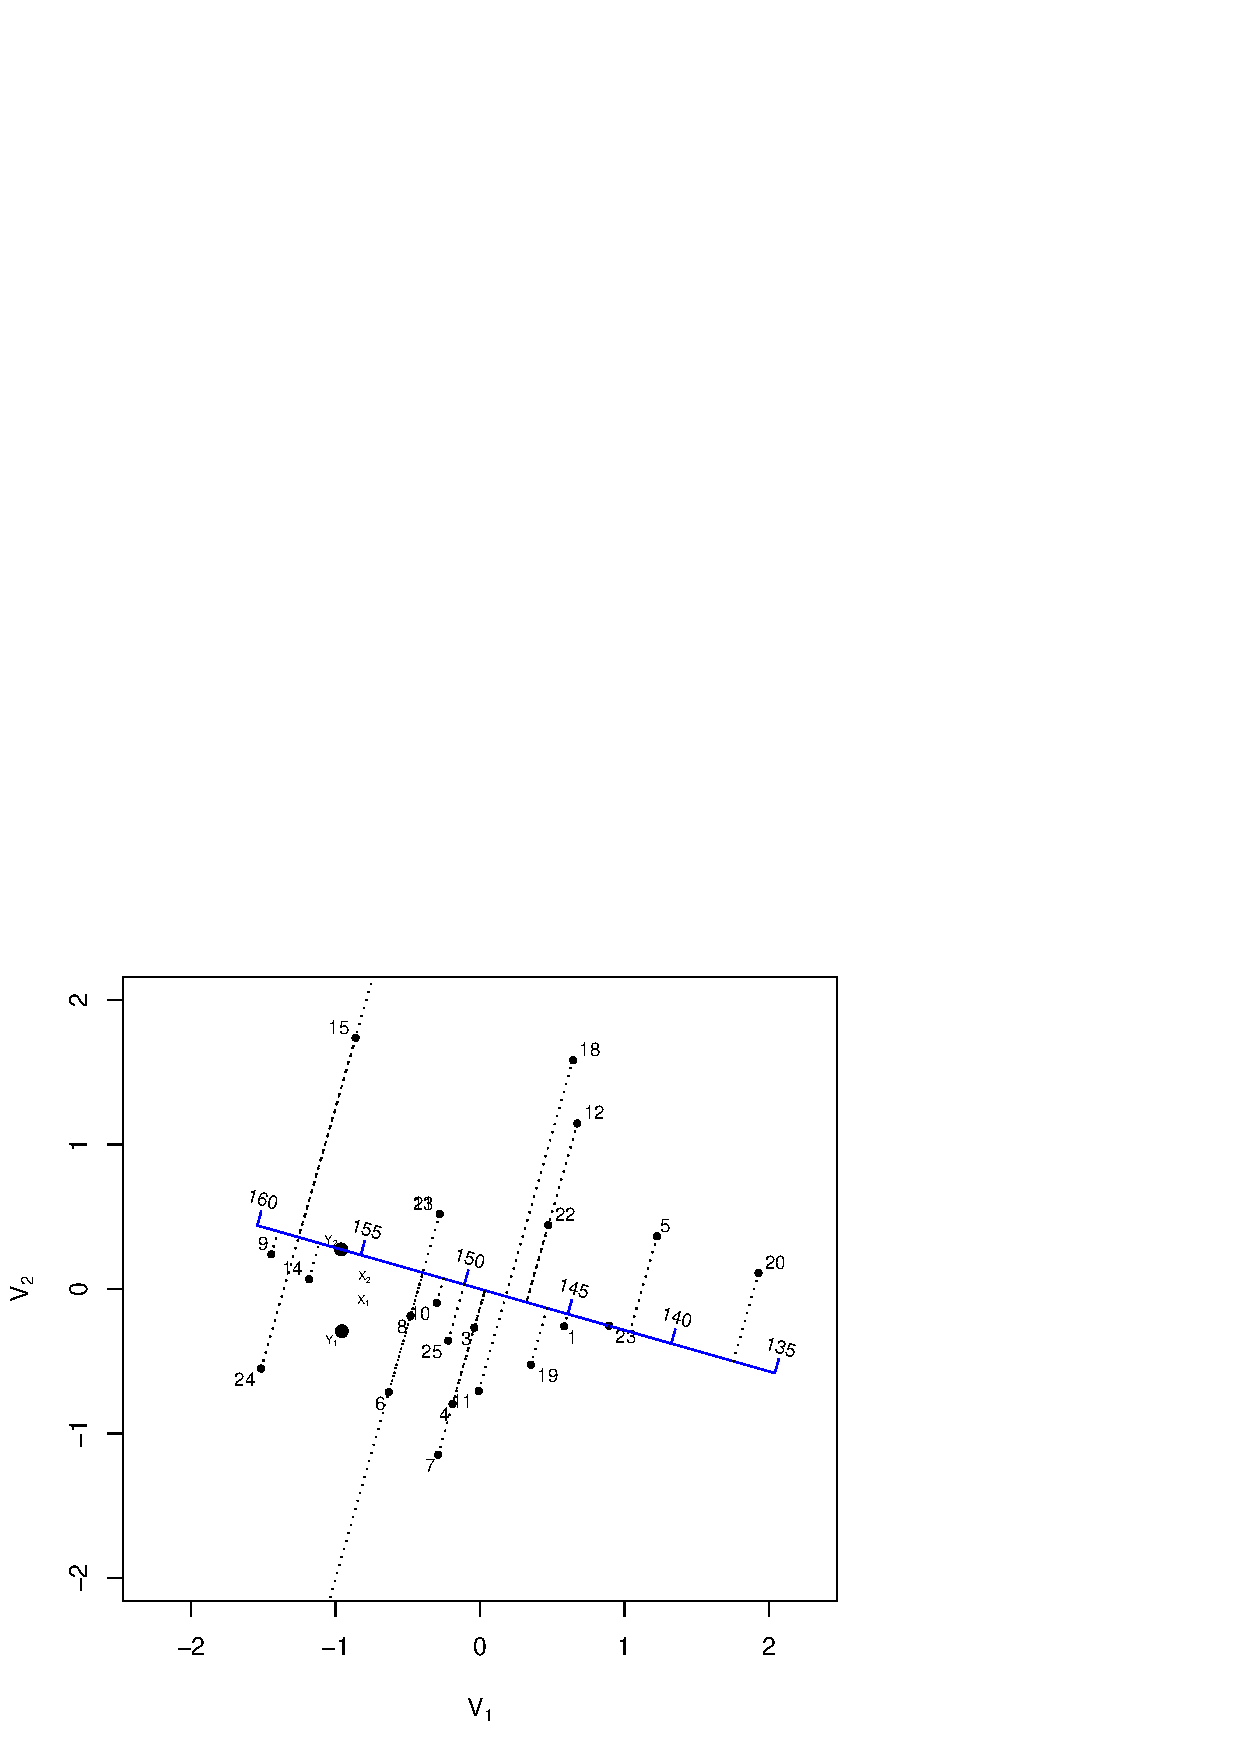
\includegraphics{CalibrationGuide-015}

We construct the biplot of the between-set correlation matrix (the joint 
plot of ${\bF}_p$ and ${\bG}_s$). 
Firstly we calibrate the biplot axis for $Y_2$ with a correlation scale.
This calibration is done by generalised least squares with the inverse of the correlation matrix of 
the X-variables as a weight matrix ({\tt weights=solve(Rxx)}). Secondly, we calibrate the biplot axis 
for $Y_2$ with a scale for the original values. This second calibration has no weight 
matrix and is obtained by ordinary least squares. Both calibrations have a goodness of fit of 1 and
allow perfect recovery of correlations and original data values.

\subsection{Redundancy analysis}
\label{sec:rda}

Redundancy analysis can be seen as a constrained PCA. It allows two biplots, the biplot of the fitted
values and a biplot of regression coefficients. Function {\tt rda} of the package provides a routine
for redundancy analysis. We use Linnerud's data on physical exercise and body measurement variables
to illustrate calibrated biplots in redundancy analysis.

\begin{Schunk}
\begin{Sinput}
> data(linnerud)
> X <- linnerud[, 1:3]
> Y <- linnerud[, 4:6]
> rda.results <- rda(X, Y)
> plot(rda.results$Fs[, 1], rda.results$Fs[, 2], 
+     pch = 16, asp = 1, xlim = c(-2, 2), ylim = c(-2, 
+         2), cex = 0.5, xlab = "1st principal axis", 
+     ylab = "2nd principal axis")
> arrows(0, 0, 2 * rda.results$Gyp[, 1], 2 * rda.results$Gyp[, 
+     2], length = 0.1)
> textxy(rda.results$Fs[, 1], rda.results$Fs[, 2], 
+     rownames(X), cx = 0.75)
> textxy(2 * rda.results$Gyp[, 1], 2 * rda.results$Gyp[, 
+     2], colnames(Y), cx = 0.75)
> y <- rda.results$Yh[, 3]
> g <- rda.results$Gyp[3, 1:2]
> Fr <- rda.results$Fs[, 1:2]
> ticklab <- c(seq(-0.6, -0.1, by = 0.1), seq(0.1, 
+     0.6, by = 0.1))
> Calibrate.Yhat3 <- calibrate(g, y, ticklab, Fr, 
+     ticklab, lm = T, dp = T, tl = 0.1, axislab = "Sauts", 
+     showlabel = F)
\end{Sinput}
\begin{Soutput}
---------- Calibration Results for  Sauts  -----------------
Length of 1 unit of the original variable =  4.3103  
Angle                                     =  46.38 degrees
Optimal calibration factor                =  18.5787  
Used calibration factor                   =  18.5787  
Goodness-of-fit                           =  0.9986  
Goodness-of-scale                         =  0.9986  
------------------------------------------------------------
\end{Soutput}
\end{Schunk}
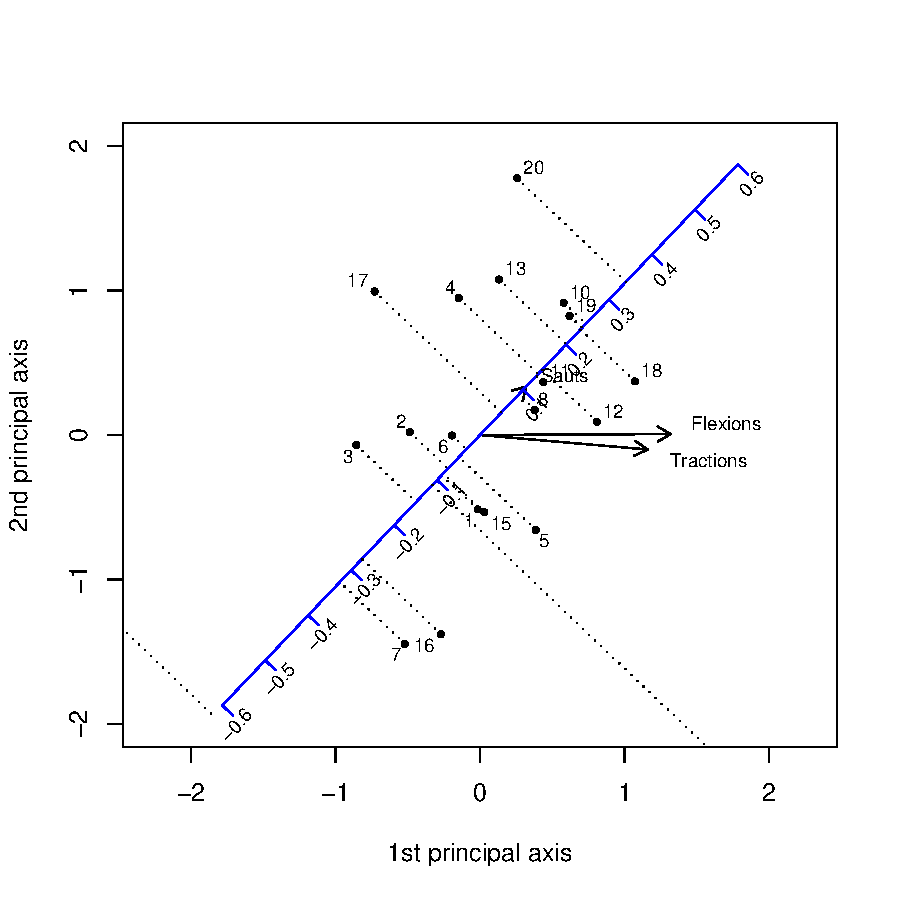
\includegraphics{CalibrationGuide-016}

\begin{Schunk}
\begin{Sinput}
> plot(rda.results$Gxs[, 1], rda.results$Gxs[, 2], 
+     pch = 16, asp = 1, xlim = c(-2, 2), ylim = c(-2, 
+         2), cex = 0.5, xlab = "1st principal axis", 
+     ylab = "2nd principal axis")
> arrows(0, 0, rda.results$Gxs[, 1], rda.results$Gxs[, 
+     2], length = 0.1)
> arrows(0, 0, rda.results$Gyp[, 1], rda.results$Gyp[, 
+     2], length = 0.1)
> textxy(rda.results$Gxs[, 1], rda.results$Gxs[, 
+     2], colnames(X), cx = 0.75)
> textxy(rda.results$Gyp[, 1], rda.results$Gyp[, 
+     2], colnames(Y), cx = 0.75)
> y <- rda.results$B[, 3]
> g <- rda.results$Gyp[3, 1:2]
> Fr <- rda.results$Gxs[, 1:2]
> ticklab <- seq(-0.4, 0.4, 0.2)
> W <- cor(X)
> Calibrate.Y3 <- calibrate(g, y, ticklab, Fr, ticklab, 
+     lm = T, dp = T, tl = 0.1, weights = W, axislab = "Sauts", 
+     showlabel = F)
\end{Sinput}
\begin{Soutput}
---------- Calibration Results for  Sauts  -----------------
Length of 1 unit of the original variable =  4.3103  
Angle                                     =  46.38 degrees
Optimal calibration factor                =  18.5787  
Used calibration factor                   =  18.5787  
Goodness-of-fit                           =  0.9986  
Goodness-of-scale                         =  0.9986  
------------------------------------------------------------
\end{Soutput}
\begin{Sinput}
> ticklab <- seq(-0.4, 0.4, 0.1)
> Calibrate.Y3 <- calibrate(g, y, ticklab, Fr, ticklab, 
+     lm = F, tl = 0.05, verb = F, weights = W)
> ticklab <- seq(-0.4, 0.4, 0.01)
> Calibrate.Y3 <- calibrate(g, y, ticklab, Fr, ticklab, 
+     lm = F, tl = 0.025, verb = F, weights = W)
\end{Sinput}
\end{Schunk}
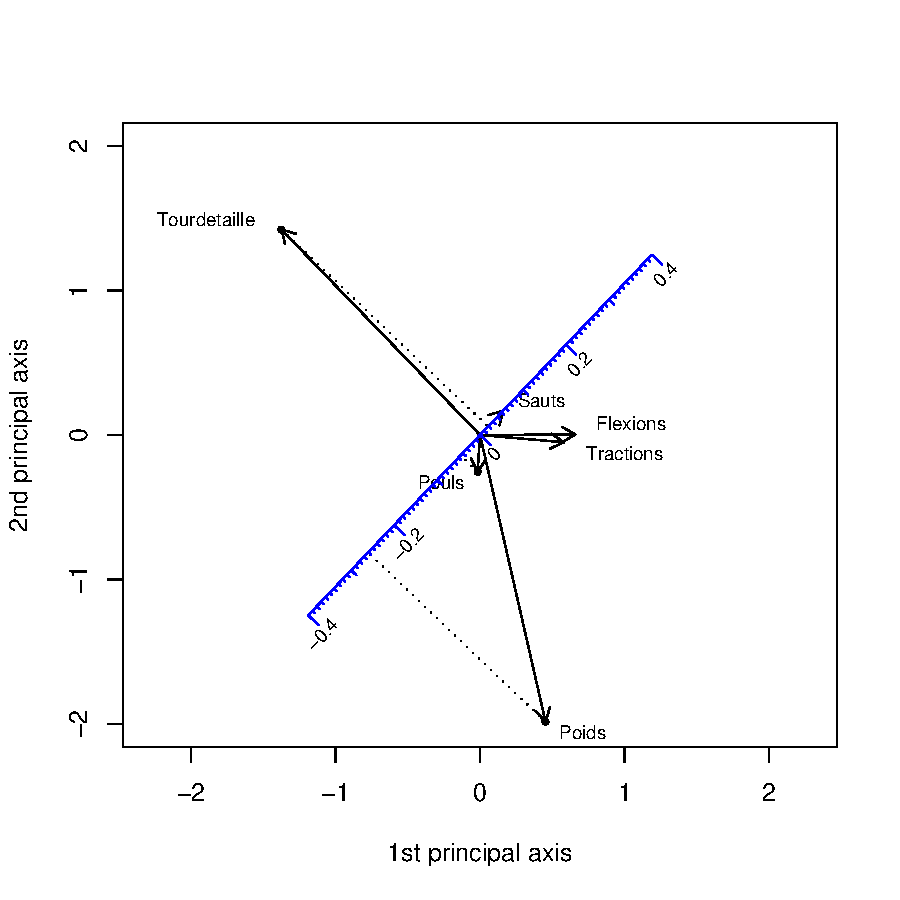
\includegraphics{CalibrationGuide-017}

The first biplot shown is a biplot of the fitted values (obtained 
from the regression of Y onto X). Vectors for the response variables are multiplied by a factor of 3 to increase
readability. The fitted values of the regression of Sauts onto the body measurements have
a goodness of fit of 0.9984 and can very well be recovered by projection onto the calibrated
axis. The second biplot is a biplot of the matrix of regression coefficients. We
calibrated the biplot axis for "Sauts", such that the regression coefficients of the
explanory variables with respect to "Sauts" can be recovered. The goodness of fit for
"Sauts" is over 0.99, which means that the regression coefficients are close to
perfectly displayed. Note that the calibration for Sauts for the regression coefficients
is done by GLS with weight matrix equal to the correlation matrix of the X variables
({\tt weights=W}).

\section{Online documentation}
\label{sec:online}

Online documentation for all routines in the package can be found in the file
{\tt calibrate.pdf} in the {\tt doc} directory of the installed package.

\section*{Acknowledgements}

This work was partially supported by the Spanish grant BEC2000-0983. I thank Holland Genetics 
({\tt http://www.hg.nl/}), Janneke van Wagtendonk and Sander de Roos for making the calves data 
available. This document was generated by Sweave~\cite{Leisch}.

\bibliographystyle{humanbio}
\begin{thebibliography}{10}

\bibitem[R Development Core Team (2004)]{RRR}
R Development Core Team 
(2004) 
R: A language and environment forstatistical computing.
R Foundation for Statistical Computing,
Vienna, Austria,
ISBN 3-900051-00-3,
http://www.R-project.org.

\bibitem[Gabriel, 1971]{Gabriel}
Gabriel, K. R. 
(1971)
The biplot graphic display of matrices with application to principal component analysis.
Biometrika 
58(3) 
pp. 453-467.

\bibitem[Graffelman and van Eeuwijk (2005)]{Graffel17}
Graffelman, J. and van Eeuwijk, F. A.,
(2005)
Calibration of multivariate scatter plots for exploratory analysis of relations within and between sets of variables 
in genomic research,
Biometrical Journal,
47,
6,
863-879.

\bibitem[Gower and Hand (1996)]{Gower4}
Gower, J. C. and Hand, D. J.
(1996)
Biplots
Chapman \& Hall,
London.

\bibitem[Manly (1989)]{Manly}
Manly, B. F. J.
(1989)
Multivariate statistical methods: a primer
Chapman and Hall, London.

\bibitem[Graffelman and Aluja-Banet (2003)]{Graffel13}
Graffelman, J. and Aluja-Banet, T.
(2003)
Optimal Representation of Supplementary Variables in Biplots from Principal Component Analysis and Correspondence Analysis
Biometrical Journal,
45(4)
pp. 491-509.

\bibitem[Venables and Ripley (2002)]{Venables}
Venables, W. N. and Ripley, B. D.
(2002)
{M}odern {A}pplied {S}tatistics with {S}-{P}lus
New York,
Fourth edition,
Springer.

\bibitem[Frets (1921)]{Frets}
Frets, G. P.
(1921)
Heredity of head form in man,
Genetica,
3, 
pp. 193-384.

\bibitem[Anderson (1984)]{Anderson}
Anderson, T. W.
(1984)
{A}n {I}ntroduction to {M}ultivariate {S}tatistical {A}nalysis
John Wiley,
Second edition,
New York.

\bibitem[Mardia et al.(1979)]{Mardia}
Mardia, K. V. and Kent, J. T. and Bibby, J. M.
(1979)
Multivariate Analysis
Academic Press London.


\bibitem[Graffelman (2005)]{Graffel16}
Graffelman, J.
(2005)
Enriched biplots for canonical correlation analysis
Journal of Applied Statistics
32(2)
pp. 173-188.


\bibitem[Leisch (2002)]{Leisch}
Leisch, F.
(2002)
Sweave: Dynamic generation of statistical reports using literate data analysis
Compstat 2002, Proceedings in Computational Statistics
pp. 575-580,
Physica Verlag, Heidelberg,
ISBN 3-7908-1517-9
URL http:/www.ci.tuwien.ac.at/~leisch/Sweave.

\end{thebibliography}

\end{document}
